{\color{gray}\hrule}
\begin{center}
\section{Implémentation}
\textbf{Dans cette section, nous verrons l'implémentation des couches de 
Pooling et de Convolution à l'aide de NumPy.}
\bigskip
\end{center}
{\color{gray}\hrule}
\begin{multicols}{2}

Il existe diverses façons de réaliser un Pooling et une Convolution
en Python. La méthode la plus intuitive consiste à parcourir chaque pixel d’une
image avec des boucles, enregistrer les informations dans des listes, puis
effectuer les calculs élément par élément. Cependant, cette approche
s’avère très lente pour des opérations complexes sur plusieurs dimensions. \\

En effet, Python est un langage interprété, ce qui signifie que chaque
ligne de code est traduite en instructions machine à l’exécution.
Cela engendre une surcharge importante, surtout lorsque des boucles répétitives
traitent un grand volume de données. Ce manque d’efficacité devient rapidement problématique
avec des images de grande taille ou des ensembles volumineux. \\

Voici ci-dessous les résultats de calculs montrant la différence de temps entre une
méthode naïve et l’utilisation de NumPy pour effectuer un produit matriciel.\\

\renewcommand{\arraystretch}{1.5}

\scalebox{0.85}{
\begin{tabular}{l|c|r} 
\textbf{Dims de A} & \textbf{Dims de B} & \textbf{Rapport de temps}\\
$$ & $$ & $t_{1}$/$t_{2}$ \\
\hline
($10^{2}, 10^{1}$) & ($10^{1}, 10^{2}$) & $\frac{0.029}{0.00046}=63.04$\\
($10^{3}, 10^{2}$) & ($10^{2}, 10^{3}$) & $\frac{10.65}{0.07}=152.14$\\
($10^{3}, 10^{3}$) & ($10^{3}, 10^{3}$) & $\frac{124.64}{0.6}=207.73$\\
\end{tabular}
}\\

\captionof{table}{Comparaison des temps de calcul pour le produit matriciel entre les matrices A et B}

{\scriptsize
$t1$ le temps de calcul avec des boucles en secondes\\
$t2$ le temps de calcul avec NumPy en secondes\\
}

On vois dans Table 1 à la ligne 3, qu'il a fallu 2 minutes à la méthode naïve pour calculer 
le produit matriciel entre A et B contre 0,6 secondes pour NumPy.\\

L’utilisation de NumPy est donc à privilégier pour accélérer les calculs tensoriels. 
En effet, la bibliothèque est implémentée en C, ce qui permet d'effectuer des
opérations directement en langage machine. Le papier \textit{"The NumPy array: a structure for efficient numerical computation"}\cite{NumPyEfficiency}
explique bien son fonctionnement et le secret de cette rapidité.

\subsection{La méthode Im2Col}

Im2Col (image to column) est une méthode de vectorisation introduite en 2006 par 
trois chercheurs de l’Inria \cite{im2col}. Cette technique convertit les tenseurs 
d’images en matrices tout en les décomposant en fenêtres, ce qui simplifie les calculs 
de convolution et de pooling tout en s’intégrant naturellement avec NumPy. \\

L'opération se présente de la manière suivante :\\

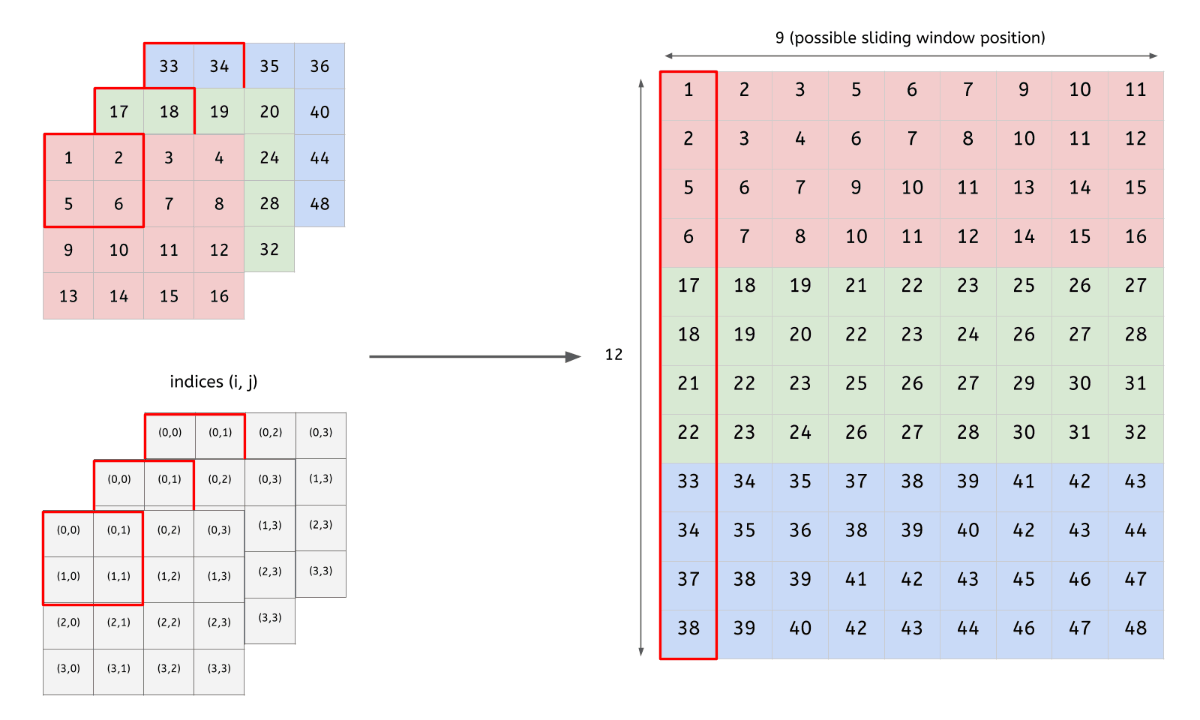
\includegraphics[width=\columnwidth]{images/im2col-1.png}
\captionof{figure}{Transformation en matrice d'une image RGB\cite{im2colImages}}
\hfill\break

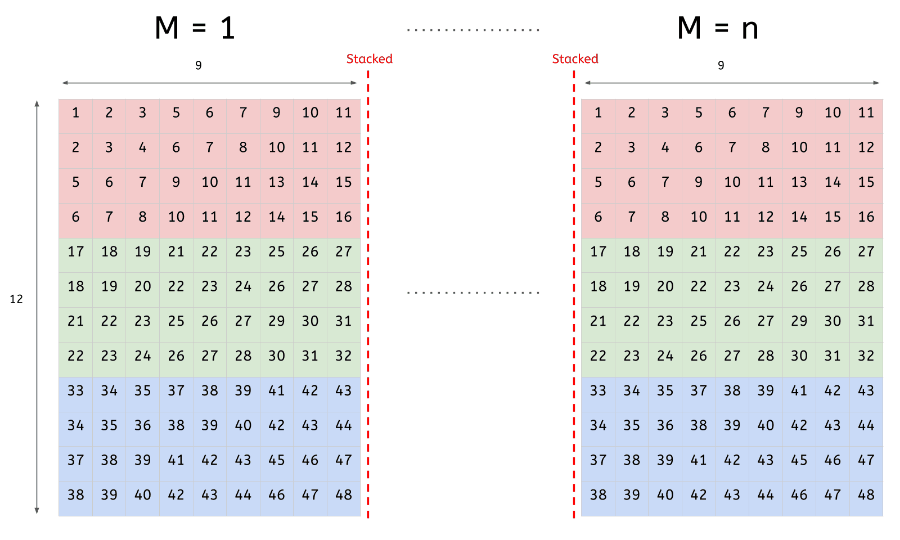
\includegraphics[width=\columnwidth]{images/im2col-2.png}
\captionof{figure}{Transformation en matrice de $n$ images RGB\cite{im2colImages}}
\hfill\break

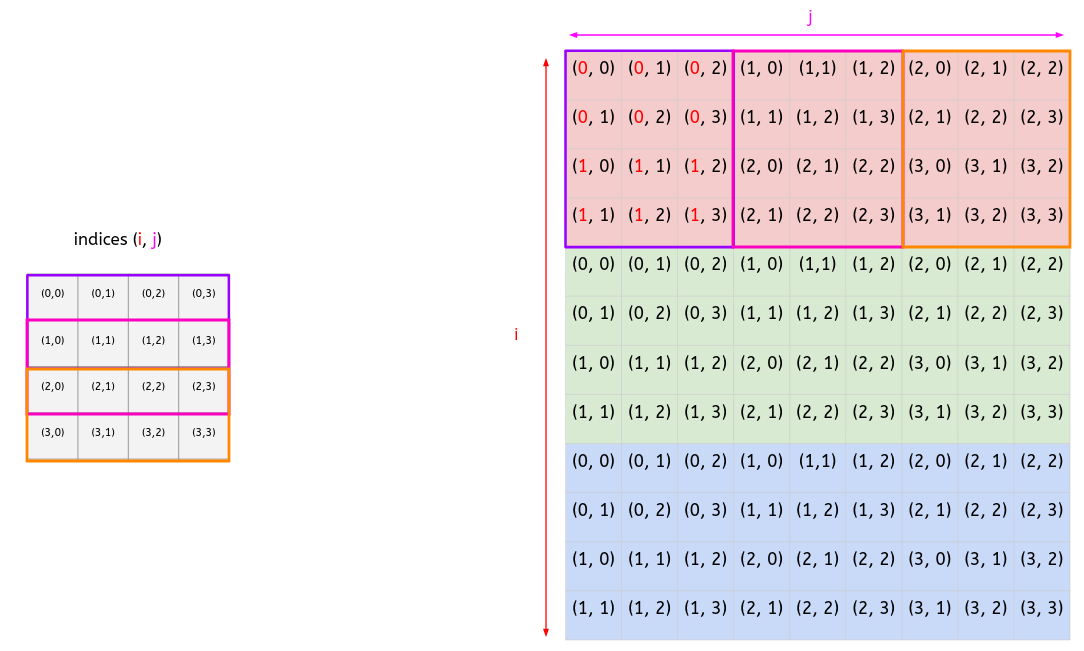
\includegraphics[width=\columnwidth]{images/im2col-3.png}
\captionof{figure}{Valeurs de la matrice remplacées par leurs indices dans l'image\cite{im2colImages}}
\hfill\break

Dans cet exemple, nous utilisons un $stride$ de 1 et une taille de fenêtre de valeur 2. 
Comme illustré dans les Figures 6, 7 et 8, les canaux d’une image sont 
concaténés verticalement (de haut en bas), tandis que les fenêtres sont 
disposées horizontalement (de gauche à droite). De même, chaque image est 
concaténée horizontalement. \\

Nous avons, dans la Figure 8, remplacé les valeurs des pixels par leur position dans 
l’image, révélant ainsi des motifs récurrents. Ces motifs nous aideront à 
générer les indices $i$, $j$ et $k$ nécessaires pour construire la matrice à 
partir des positions des pixels. Examinons ces motifs en détail et 
modélisons-les mathématiquement. \\

Ici, le motif de l’indice $i$ au niveau 1 (zone violette dans la Figure 8) est $ (0,0,1,1) $. 
On remarque ensuite que les éléments sont additionnés par 1 au niveau 2 (zone rose dans la Figure 8) 
puis additionnés une nouvelle fois au niveau 3 (zone orange dans la Figure 8). Nous pouvons donc généraliser 
avec la formule suivante : \\

$ i_{m} = \{0_{0}+(m-1)\times stride,0_{1}+(m-1)\times stride,...,0_{k-1}+(m-1)\times stride, 1_{0}+(m-1)\times stride,1_{1}+(m-1)\times stride,...,1_{k-1}+(m-1)\times stride, (k-1)_{0}+(m-1)\times stride, (k-1)_{1}+(m-1)\times stride,..., (k-1)_{k-1}+(m-1)\times stride \}$,
où $m$ correspond au niveau, à partir de $m=1$ et $k$ la taille de la fenêtre. \\

Voici le code Python nécessaire pour générer les indices $i$ : \\

\begin{lstlisting}[language=Python]
import numpy as np

level1 = np.repeat(np.arange(window_shape), window_shape)
level1 = np.tile(level1, image_shape[1])

increment = stride * np.repeat(np.arange(output_height), output_width)

i = level1.reshape(-1, 1) + increment.reshape(1, -1)
\end{lstlisting} 
\hfill\break

Dans la ligne 3, \texttt{np.arrange(window\_shape)} génère une séquence d'entiers allant 
de 0 à \texttt{window\_shape-1} et \texttt{np.repeat(..., window\_shape)}
répète chaque élément de cette séquence un nombre de fois égal à \texttt{window\_shape}. \\

Dans la ligne 4, \texttt{np.tile(level1, image\_shape[1])} répète tout le tableau 
\texttt{level1} horizontalement un nombre de fois égal au nombre de canaux. \\

Dans la ligne 6, \texttt{np.arange(output\_height)} génère une séquence d’entiers allant
de 0 à \texttt{output\_height-1} et \texttt{np.repeat(..., output\_width)} répète chaque entier
de cette séquence un nombre de fois égal à \texttt{output\_width}. Ensuite, le résultat
est multiplié par le $stride$. \\

Dans la ligne 8, \texttt{level1.reshape(-1, 1)} transforme le tableau level1 en un
vecteur colonne. De même, \texttt{increment.reshape(1, -1)} transforme le tableau \texttt{increment} en un vecteur 
ligne. L’addition entre ces deux matrices suit les règles de broadcasting de NumPy\cite{NumPyEfficiency}, 
combinant chaque élément de \texttt{level1} avec chaque élément de increment pour produire une matrice
contenant l'ensemble des indices $i$. \\

Concernant l’indice $j$, les motifs observés sont : 
$j_{1,2,3} = \{(0,1,0,1),(1,2,1,2),(2,3,2,3)\}$. On voit qu'à chaque déplacement 
de la fenêtre, les indices $j$ sont additionnés par 1 à partir de $j_{1}$. On peut donc généraliser
de la manière suivante : \\

$j_{n} = \{0_{0}+(n-1) \times stride,1_{0}+(n-1)\times stride,...,(k-1)_{0}+(n-1)\times stride,...,0_{k-1}+(n-1)\times stride,1_{k-1}+(n-1)\times stride,...,(k-1)_{k-1}+(n-1)\times stride\}$\\
où $n$ correspond au glissement, à partir de $n=1$ et $k$ la taille de la fenêtre. \\

Voici le code Python nécessaire pour générer les indices $j$ : \\

\begin{lstlisting}[language=Python]
import numpy as np

slide1 = np.tile(np.arange(window_shape), window_shape * image_shape[1])
increment = stride * np.tile(np.arange(output_width), output_height)

j = slide1.reshape(-1, 1) + increment.reshape(1, -1)
\end{lstlisting}
\hfill\break

Dans la ligne 3, \texttt{np.arange(window\_shape)} génère une séquence d’entiers allant
de 0 à \texttt{window\_shape-1} et \texttt{np.repeat(..., window\_shape)} répète chaque élément
de cette séquence un nombre de fois égal à \texttt{window\_shape}. \\

Dans la ligne 4, \texttt{np.tile(level1, image\_shape[1])} répète tout le tableau
level1 horizontalement un nombre de fois égal au nombre de canaux. \\

Dans la ligne 6, \texttt{np.arange(output\_height}) génère une séquence d’entiers allant
de 0 à \texttt{output\_height-1} et \texttt{ np.repeat(..., output\_width)} répète chaque entier
de cette séquence un nombre de fois égal à \texttt{output\_width}. Ensuite, le résultat
est multiplié par le $stride$. \\

Dans la ligne 8, \texttt{slide1.reshape(-1, 1)} transforme le tableau \texttt{slide1} en un
vecteur colonne. De même, \texttt{increment.reshape(1, -1)} transforme le tableau \texttt{increment} en un vecteur
ligne. L’addition entre ces deux matrices suit, encore une fois, les règles de broadcasting de NumPy\cite{NumPyEfficiency},
combinant chaque élément de slide1 avec chaque élément de increment pour produire
une matrice contenant l’ensemble des indices $j$. \\

Concernant l’indice des canaux  $k$, il suffit de répéter les indices des canaux pour 
chaque pixel dans une fenêtre. \\

Voici le code Python nécessaire pour générer les indices $k$ : \\

\begin{lstlisting}[language=Python]
import numpy as np

k = np.repeat(np.arange(image_shape[1]), window_shape * window_shape).reshape(-1, 1)  
\end{lstlisting}
\hfill\break

Dans cette ligne, \texttt{np.arange(image\_shape[1])} génère une séquence d’entiers allant
de 0 au nombre de canaux de l’image. Ensuite, \texttt{np.repeat(..., window\_shape * window\_shape)} répète chaque entier de 
cette séquence un nombre de fois égal à \texttt{window\_shape * window\_shape}, c’est-à-dire le nombre de pixels dans une fenêtre.
Enfin, \texttt{.reshape(-1, 1)} transforme le tableau résultant en un vecteur colonne, contenant l'ensemble
des indices $k$. \\

Maintenant que nous avons les indices, il reste à générer la matrice 
correspondant au jeu de données :\\

\begin{lstlisting}[language=Python]
import numpy as np

k, i, j = get_indices(images.shape, window_shape, stride)
columns = np.concatenate(images[:, k, i, j], axis=-1)
\end{lstlisting}

Dans ce code, chaque image est vectorisée puis concaténée avec les précédentes. 
À la fin, nous obtenons des colonnes de matrices correspondant à chacune d'entre elles. \\

L'opération inverse (Col2Im) est également possible en replaçant chaque pixel 
à sa position initiale :

\begin{lstlisting}[language=Python]
import numpy as np

images = np.zeros(image_shape)
k, i, j = get_indices(image_shape, window_shape, stride)
cols_reshaped = np.array(np.hsplit(columns, image_shape[0]))
np.add.at(images, (slice(None), k, i, j), cols_reshaped)
\end{lstlisting}

Dans le cas où le $stride$ crée des fenêtres qui se superposent,
les pixels sont additionnés aux positions concernées (voir Figure 9). Cela n'aura pas 
d'effets négatifs dans nos calculs étant donné que cela réspecte leur 
contribution.\\

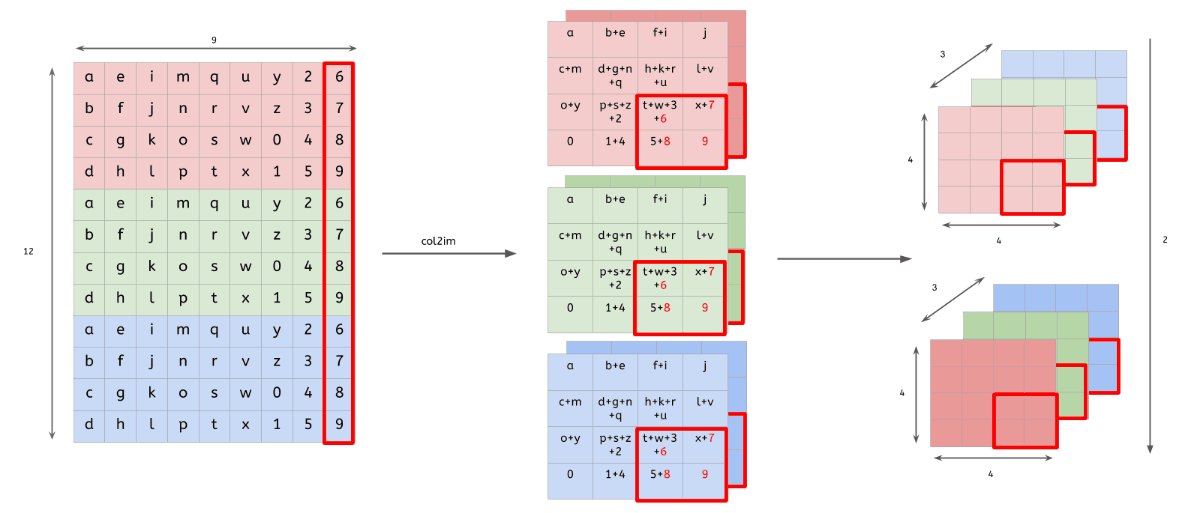
\includegraphics[width=\columnwidth]{images/im2col-4.png}
\captionof{figure}{Opération Col2Im\cite{im2colImages}}
\hfill\break

L'ensemble du code de la méthode Im2col se trouve dans le repo de Melpy,
à l'adresse suivante : \url{https://github.com/lennymalard/melpy-project/blob/main/melpy/im2col.py}

\subsection{Les couches de Convolution}

Les couches $Convolution2D$ héritent de la superclasse $Layer$ 
de Melpy, ce qui leur impose l’utilisation des méthodes 
\textbf{forward()} et \textbf{backward()} pour effectuer 
respectivement les propagations avant et arrière.\\

Voici, dans un premier temps, le code de la propagation avant :\\

\begin{lstlisting}[language=Python]
def forward(self):
    self.input_padded = self.explicit_padding()

    self.input_cols = im2col(self.input_padded, self.kernel_size, self.stride)
    self.filter_cols = self.weights.reshape(self.out_channels, -1)

    output_height, output_width = self.get_output_size(self.inputs.shape[2], self.inputs.shape[3])

    self.output_cols = self.filter_cols @ self.input_cols

    self.outputs = np.array(np.hsplit(self.output_cols, self.inputs.shape[0])).reshape(
        (self.input_padded.shape[0], self.out_channels, output_height, output_width)
    )

    if self.biases is not None:
        self.outputs += self.biases

    return self.outputs
\end{lstlisting}
\hfill\break

Les images d’entrée sont d’abord paddées via \texttt{self.explicit\_padding()} pour ajuster leurs dimensions, 
puis converties en colonnes avec \texttt{im2col()}. Les poids de la couche sont également aplatis en une 
matrice pour pouvoir effectuer un produit matriciel avec les colonnes d’images. Les dimensions de sortie sont 
calculées avec \texttt{self.get\_output\_size()}, et la convolution est réalisée en multipliant les colonnes des images 
par les filtres aplatis. Les résultats sont réassemblés en images, ajustés si des biais sont 
présents, puis retournés comme résultats finaux de la couche pour être propagés en avant.\\

Voici maintenant le code de la propagation arrière : \\

\begin{lstlisting}[language=Python]
def backward(self, dX):
    self.dY = dX

    flipped_filters = self.weights[:, :, ::-1, ::-1]
    flipped_filters_cols = flipped_filters.reshape(self.out_channels, -1)

    self.dY_reshaped = self.dY.reshape(self.dY.shape[0] * self.dY.shape[1], self.dY.shape[2] * self.dY.shape[3])
    self.dY_reshaped = np.array(np.vsplit(self.dY_reshaped, self.inputs.shape[0]))
    self.dY_reshaped = np.concatenate(self.dY_reshaped, axis=-1)

    self.dX_cols = flipped_filters_cols.T @ self.dY_reshaped
    self.dW_cols = self.dY_reshaped @ self.input_cols.T

    self.dX_padded = col2im(self.dX_cols, self.input_padded.shape, self.kernel_size, self.stride)

    if self.padding == "same":
        (pad_top, pad_bottom, pad_left, pad_right) = self.calculate_padding()
        self.dX = self.dX_padded[:, :, pad_top:-pad_bottom, pad_left:-pad_right]
    else:
        self.dX = self.dX_padded

    self.dW = self.dW_cols.reshape((self.dW_cols.shape[0], self.in_channels, self.kernel_size, self.kernel_size))

    if self.biases is not None:
        self.dB = np.sum(self.dY, axis=(0, 2, 3), keepdims=True)

    return self.dX
\end{lstlisting}
\hfill\break

Les gradients de sortie \texttt{dX} sont assignés à \texttt{self.dY}, et les filtres sont 
retournés de \ang{180} puis aplatis en colonnes pour les calculs. Les gradients \texttt{self.dY} 
sont convertis en colonnes, et les gradients des entrées \texttt{self.dX} sont calculés 
via un produit matriciel entre les colonnes des filtres retournés et $dY$. 
Les gradients des poids \texttt{self.dW} sont quant à eux obtenus par multiplication entre $dY$ et 
les colonnes d’entrée transposées. Les gradients des biais \texttt{self.dB}, si présents, sont calculés par une somme. 
Les gradients d’entrée sont reconstitués avec \texttt{col2im()} et ajustés pour retirer le padding si nécessaire. 
Finalement, les gradients \texttt{self.dX} sont retournés pour poursuivre la propagation arrière. \\

L'ensemble du code lié aux couches de Convolution se trouvent dans le repo de Melpy, à l'adresse suivante : \url{https://github.com/lennymalard/melpy-project/blob/main/melpy/layers.py}

\subsection{Les couches de Pooling}

Les couches $Pooling2D$ héritent également de la superclasse $Layer$ 
de Melpy, leur imposant les mêmes contraintes que $Convolution2D$.\\

Voici donc le code de la propagation avant : \\

\begin{lstlisting}[language=Python]
def forward(self):
    output_height = int((self.inputs.shape[2] - self.pool_size + self.stride) // self.stride)
    output_width = int((self.inputs.shape[3] - self.pool_size + self.stride) // self.stride)

    output_shape = (self.inputs.shape[0], self.inputs.shape[1], output_height, output_width)

    self.input_cols = im2col(self.inputs, self.pool_size, self.stride)
    self.input_cols_reshaped = np.array(np.hsplit(np.array(np.hsplit(self.input_cols, self.inputs.shape[0])), self.inputs.shape[1]))

    self.maxima = np.max(self.input_cols_reshaped, axis=2)
    self.maxima_reshaped = self.maxima.reshape(self.inputs.shape[1], -1)

    self.outputs = col2im(self.maxima_reshaped, output_shape, 1, 1)

    return self.outputs
\end{lstlisting}
\hfill\break

Les dimensions de sortie sont d’abord calculées, en fonction des dimensions d’entrée, 
de la taille de la fenêtre de pooling, et du $stride$. Les entrées sont ensuite 
transformées en colonnes à l’aide de \texttt{im2col()}. Les colonnes sont restructurées pour 
correspondre aux canaux et échantillons, puis l’opération \texttt{np.max()}
extrait les maxima de chaque fenêtre. Ces valeurs maximales sont réorganisées et 
reconstruites en utilisant \texttt{col2im()} pour former les sorties finales.
Ces sorties sont finalement retournées pour poursuivre la propagation avant.\\

Voici maintenant le code de la propagation arrière : \\

\begin{lstlisting}[language=Python]
def backward(self, dX):
    self.dY = dX
    self.dX = np.zeros_like(self.inputs)

    self.dY_cols = im2col(self.dY, 1, 1)
    self.dY_cols_reshaped = np.array(np.hsplit(np.array(np.hsplit(self.dY_cols, self.dY.shape[0])), self.dY.shape[1])).transpose(0, 1, 3, 2)

    self.input_cols = im2col(self.inputs, self.pool_size, self.stride)
    self.input_cols_reshaped = np.array(np.hsplit(np.array(np.hsplit(self.input_cols, self.inputs.shape[0])), self.inputs.shape[1])).transpose(0, 1, 3, 2)

    self.output_cols = im2col(self.outputs, 1, 1)
    self.output_cols_reshaped = np.array(np.hsplit(np.array(np.hsplit(self.output_cols, self.inputs.shape[0])), self.inputs.shape[1])).transpose(0, 1, 3, 2)

    self.mask = np.array(self.input_cols_reshaped == self.output_cols_reshaped, dtype=np.uint64)

    self.dX_cols = np.concatenate(np.concatenate(np.array(self.mask * self.dY_cols_reshaped).transpose(0, 1, 3, 2), axis=1), axis=1)
    self.dX = col2im(self.dX_cols, self.inputs.shape, self.pool_size, self.stride)

    return self.dX
\end{lstlisting}
\hfill\break

Les gradients reçus \texttt{dX} sont sauvegardés dans \texttt{self.dY}, puis 
transformés en colonnes avec \texttt{im2col()}. Les entrées 
originales et les sorties de la propagation avant sont également converties en colonnes et 
restructurées. Un masque binaire identifiant les maxima des fenêtres de pooling est créé 
pour ne transmettre que les gradients associés à ces maxima. Les gradients modifiés sont 
réassemblés en une forme plate, puis reconstruits avec \texttt{col2im()} pour correspondre 
aux dimensions des entrées. Enfin, les gradients des entrées reconstitués \texttt{self.dX}
sont retournés pour continuer la propagation arrière. \\

L'ensemble du code lié aux couches de Pooling se trouvent dans le repo de Melpy, à l'adresse suivante : \url{https://github.com/lennymalard/melpy-project/blob/main/melpy/layers.py}

\end{multicols}


